\section{Auswertung}
\label{sec:Auswertung}
Es werden nun die mithilfe des digitalen Oszilloskopes ermittelten Amplituden des Ausgabesignals ausgewertet.

\subsection{Messung ohne Rauschen}
\label{sec:ohne rauschen}
In \autoref{fig:Bilder normal} sind Oszilloskopbilder von ausgewählten Phasenverschiebungen für die Messung ohne Rauschen zu sehen.

\begin{figure} [H]
  \begin{subfigure}{0.48\textwidth}
    \centering
    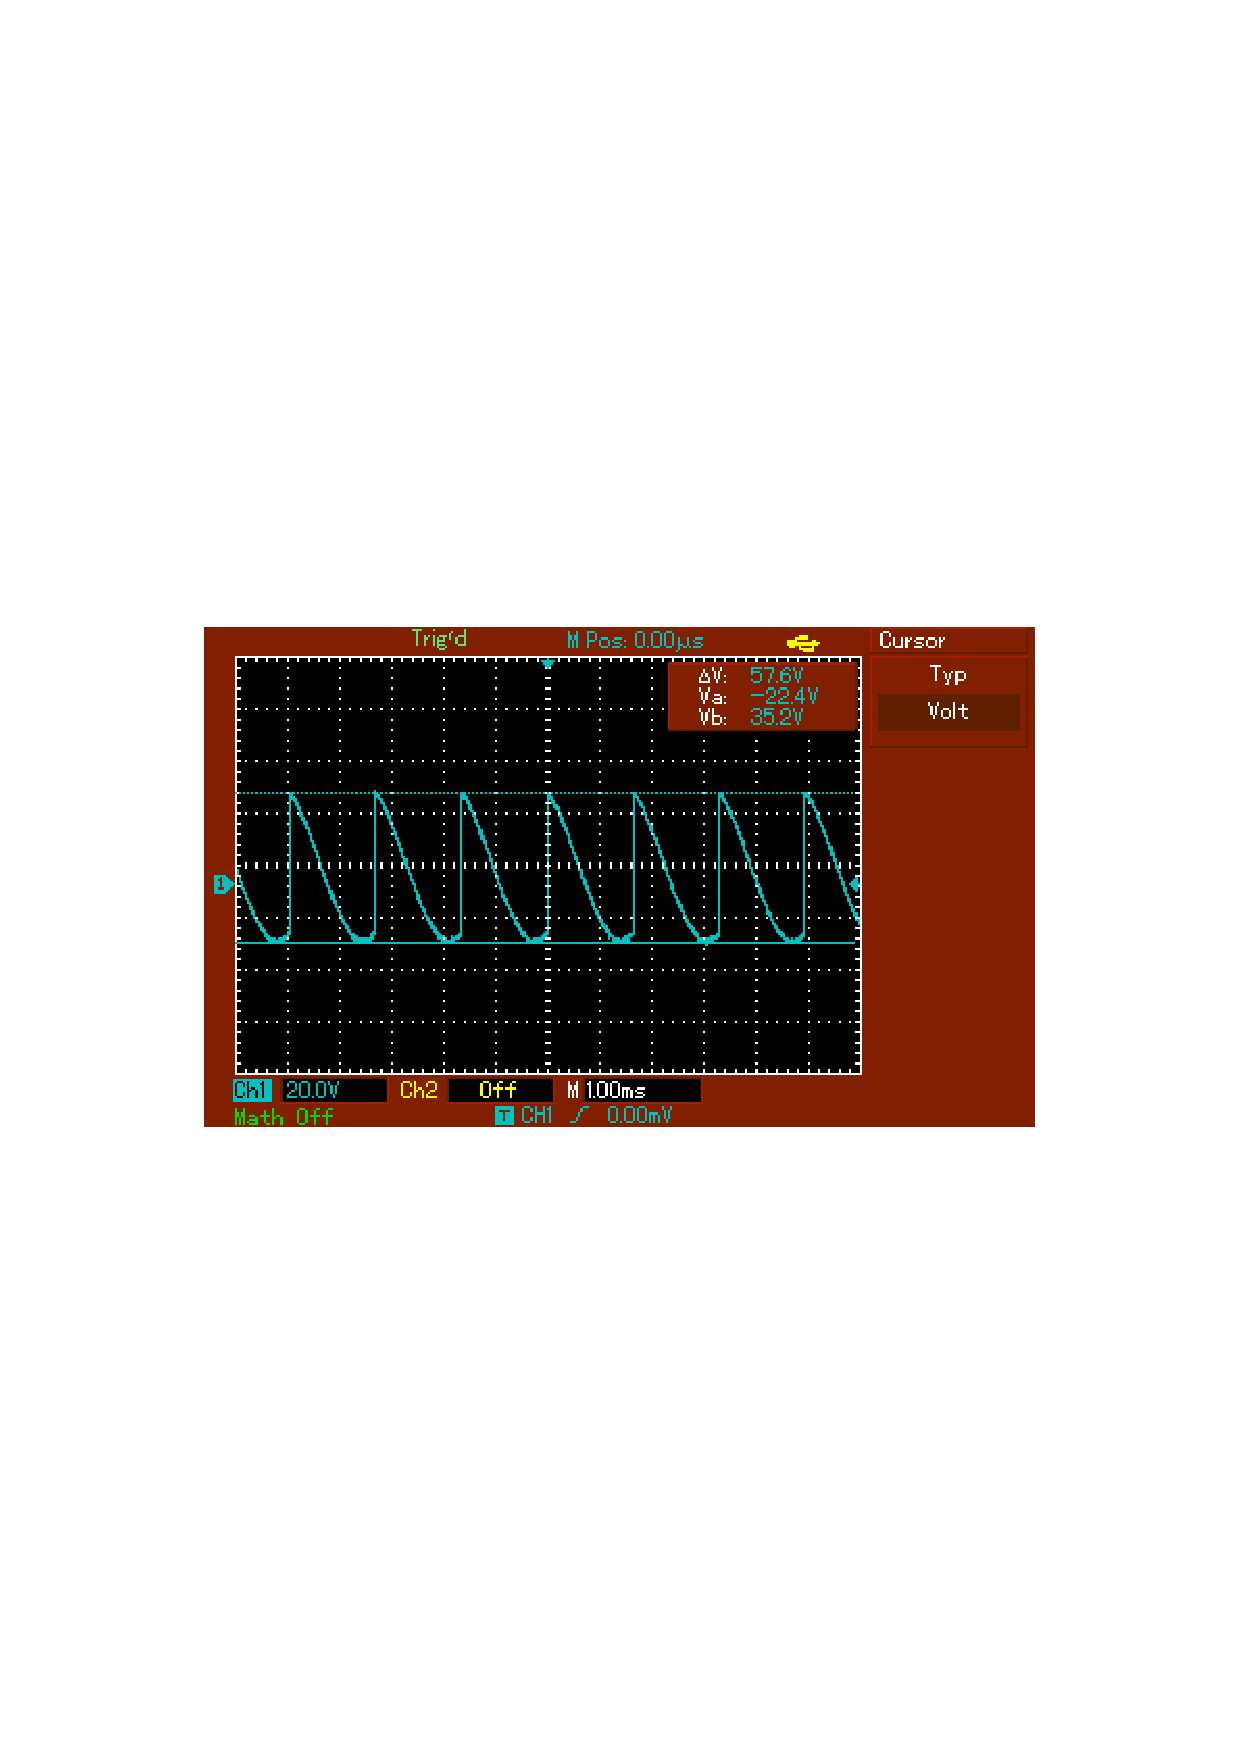
\includegraphics[height=4cm]{content/Bilder/unverrauscht/0.pdf}
    \caption{$\symup{\Delta}\varphi = \qty{0}{\degree}$}
    \label{fig:unverrauscht 0}
  \end{subfigure}
  \begin{subfigure}{0.48\textwidth}
    \centering
    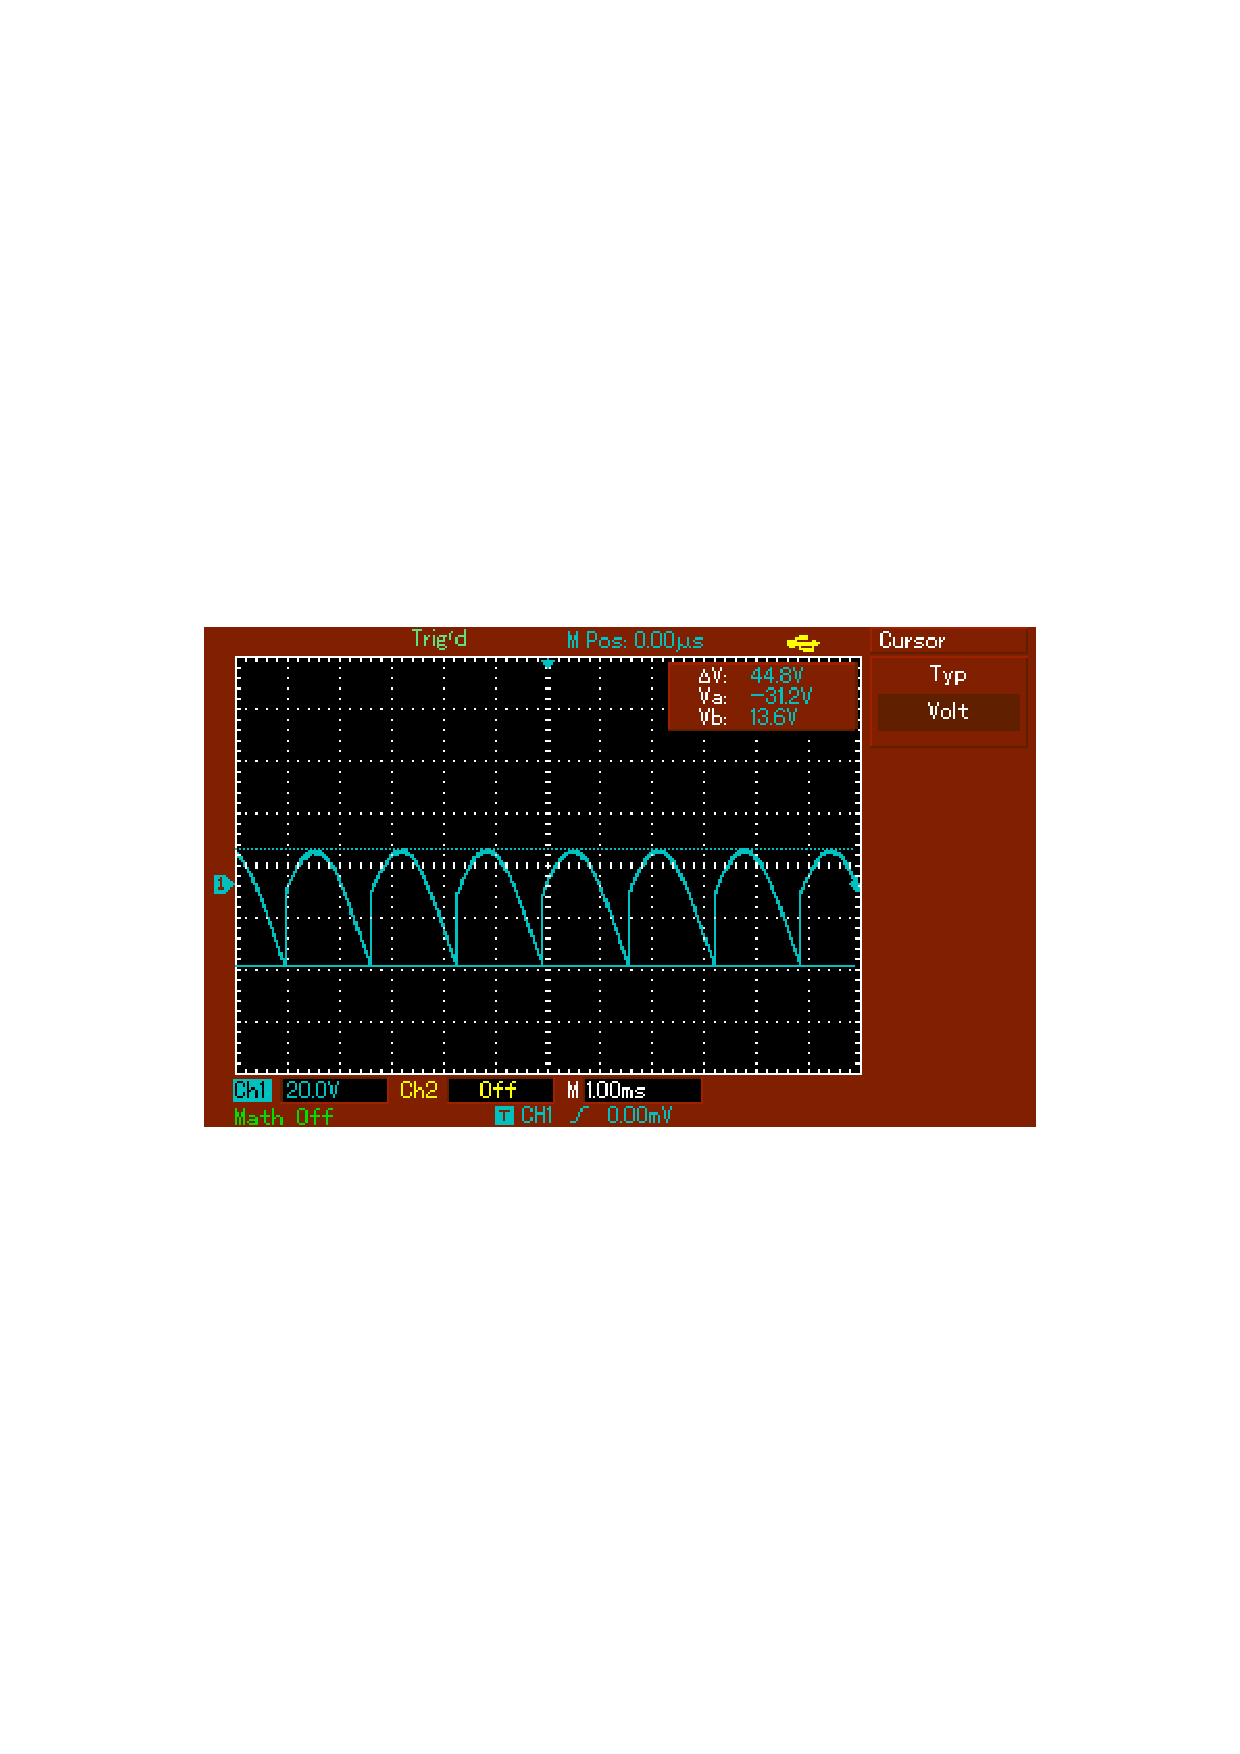
\includegraphics[height=4cm]{content/Bilder/unverrauscht/90.pdf}
    \caption{$\symup{\Delta}\varphi = \qty{90}{\degree}$}
  \end{subfigure}
  \begin{subfigure}{0.48\textwidth}
    \centering
    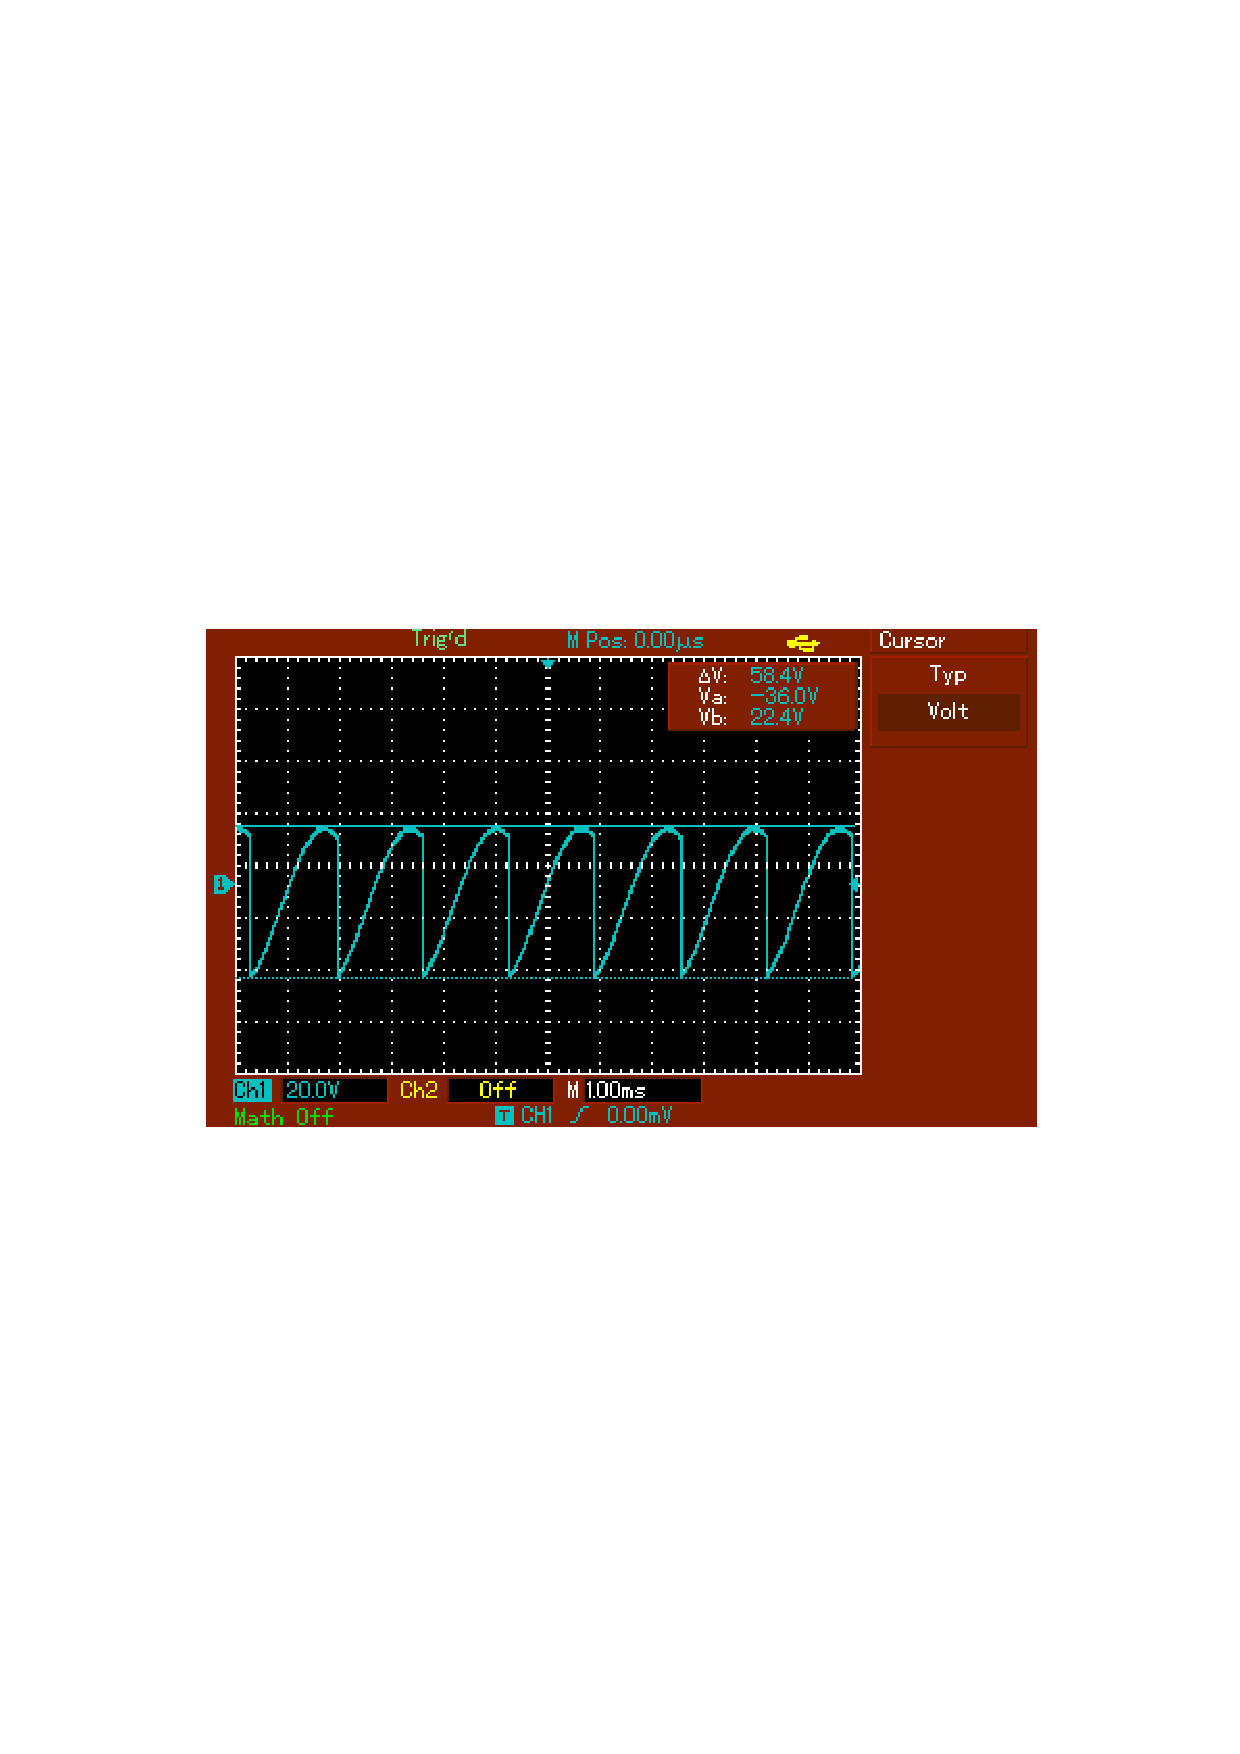
\includegraphics[height=4cm]{content/Bilder/unverrauscht/180.pdf}
    \caption{$\symup{\Delta}\varphi = \qty{180}{\degree}$}
  \end{subfigure}
  \begin{subfigure}{0.48\textwidth}
    \centering
    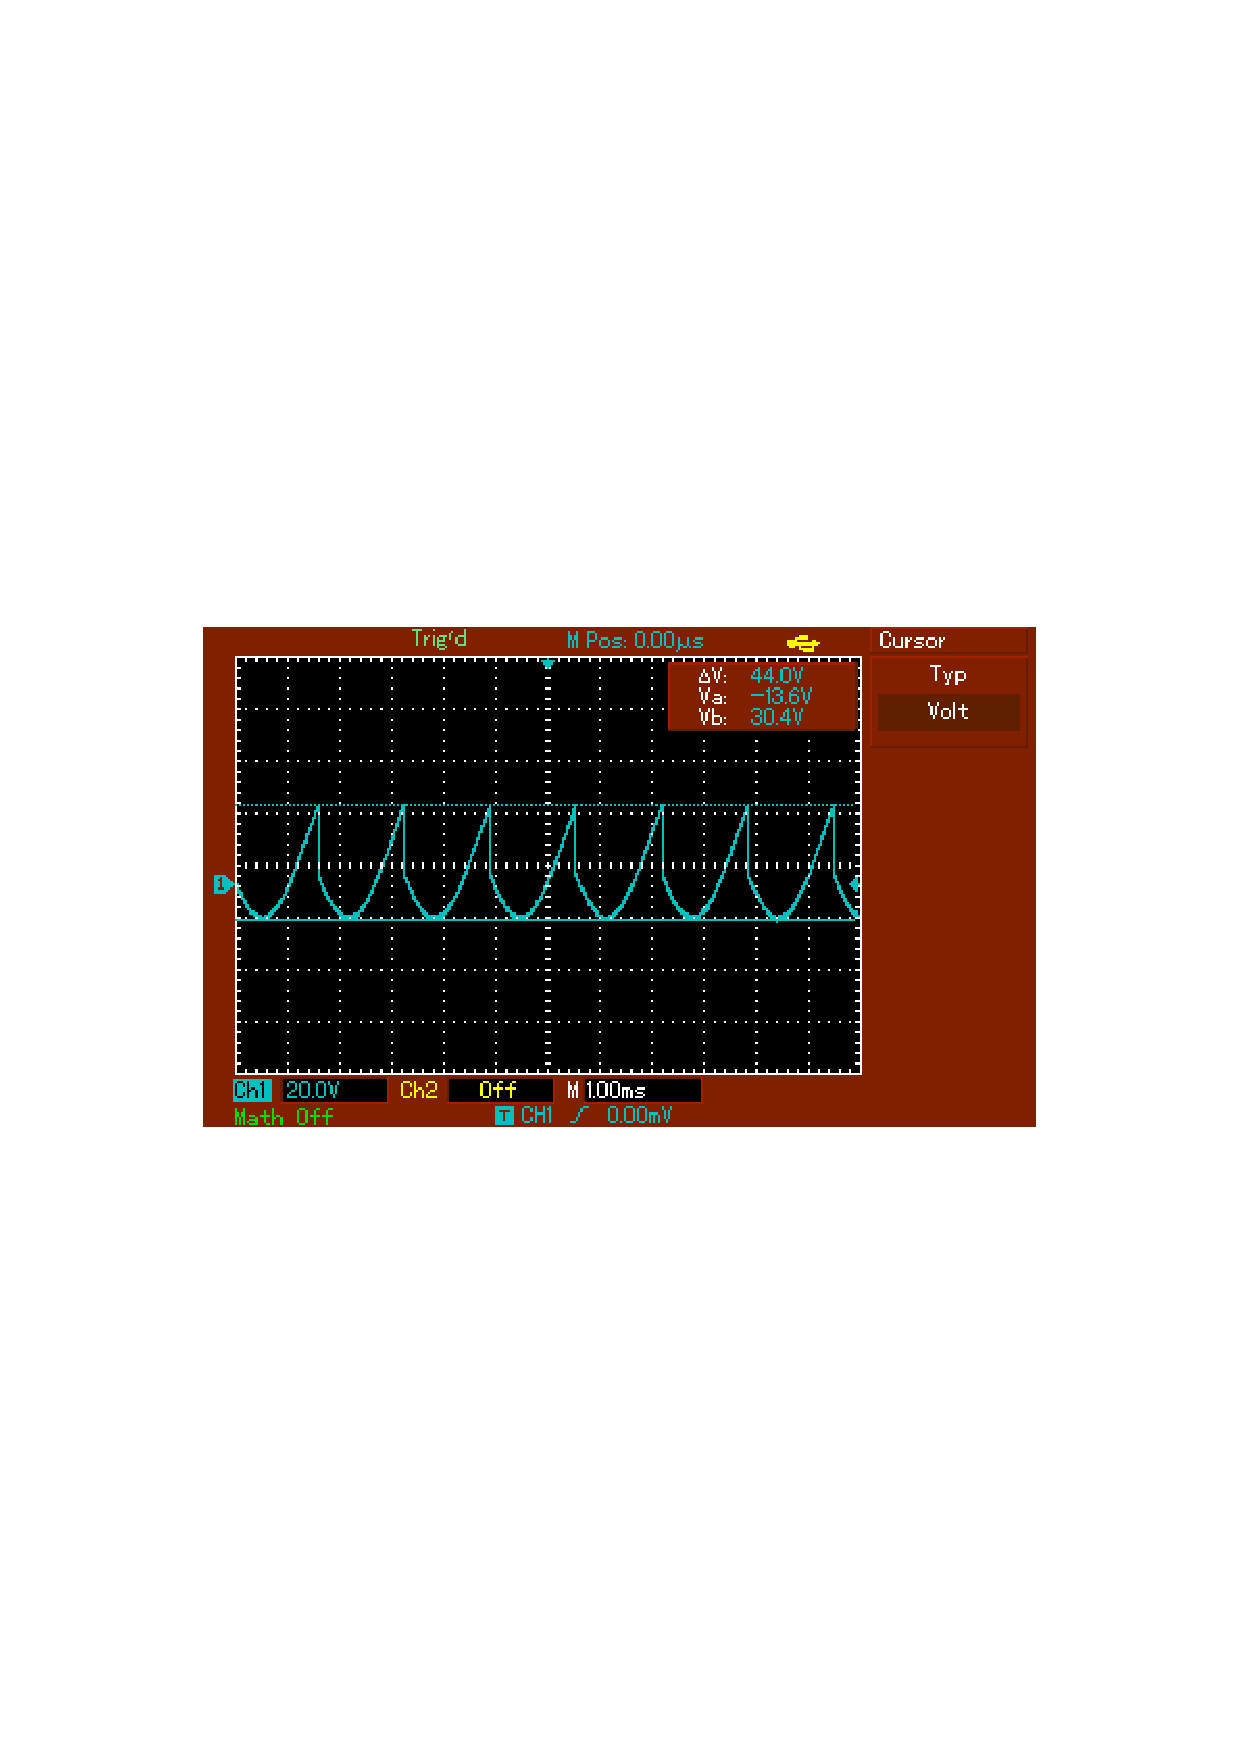
\includegraphics[height=4cm]{content/Bilder/unverrauscht/270.pdf}
    \caption{$\symup{\Delta}\varphi = \qty{270}{\degree}$}
  \end{subfigure}
  \begin{subfigure}{0.48\textwidth}
    \centering
    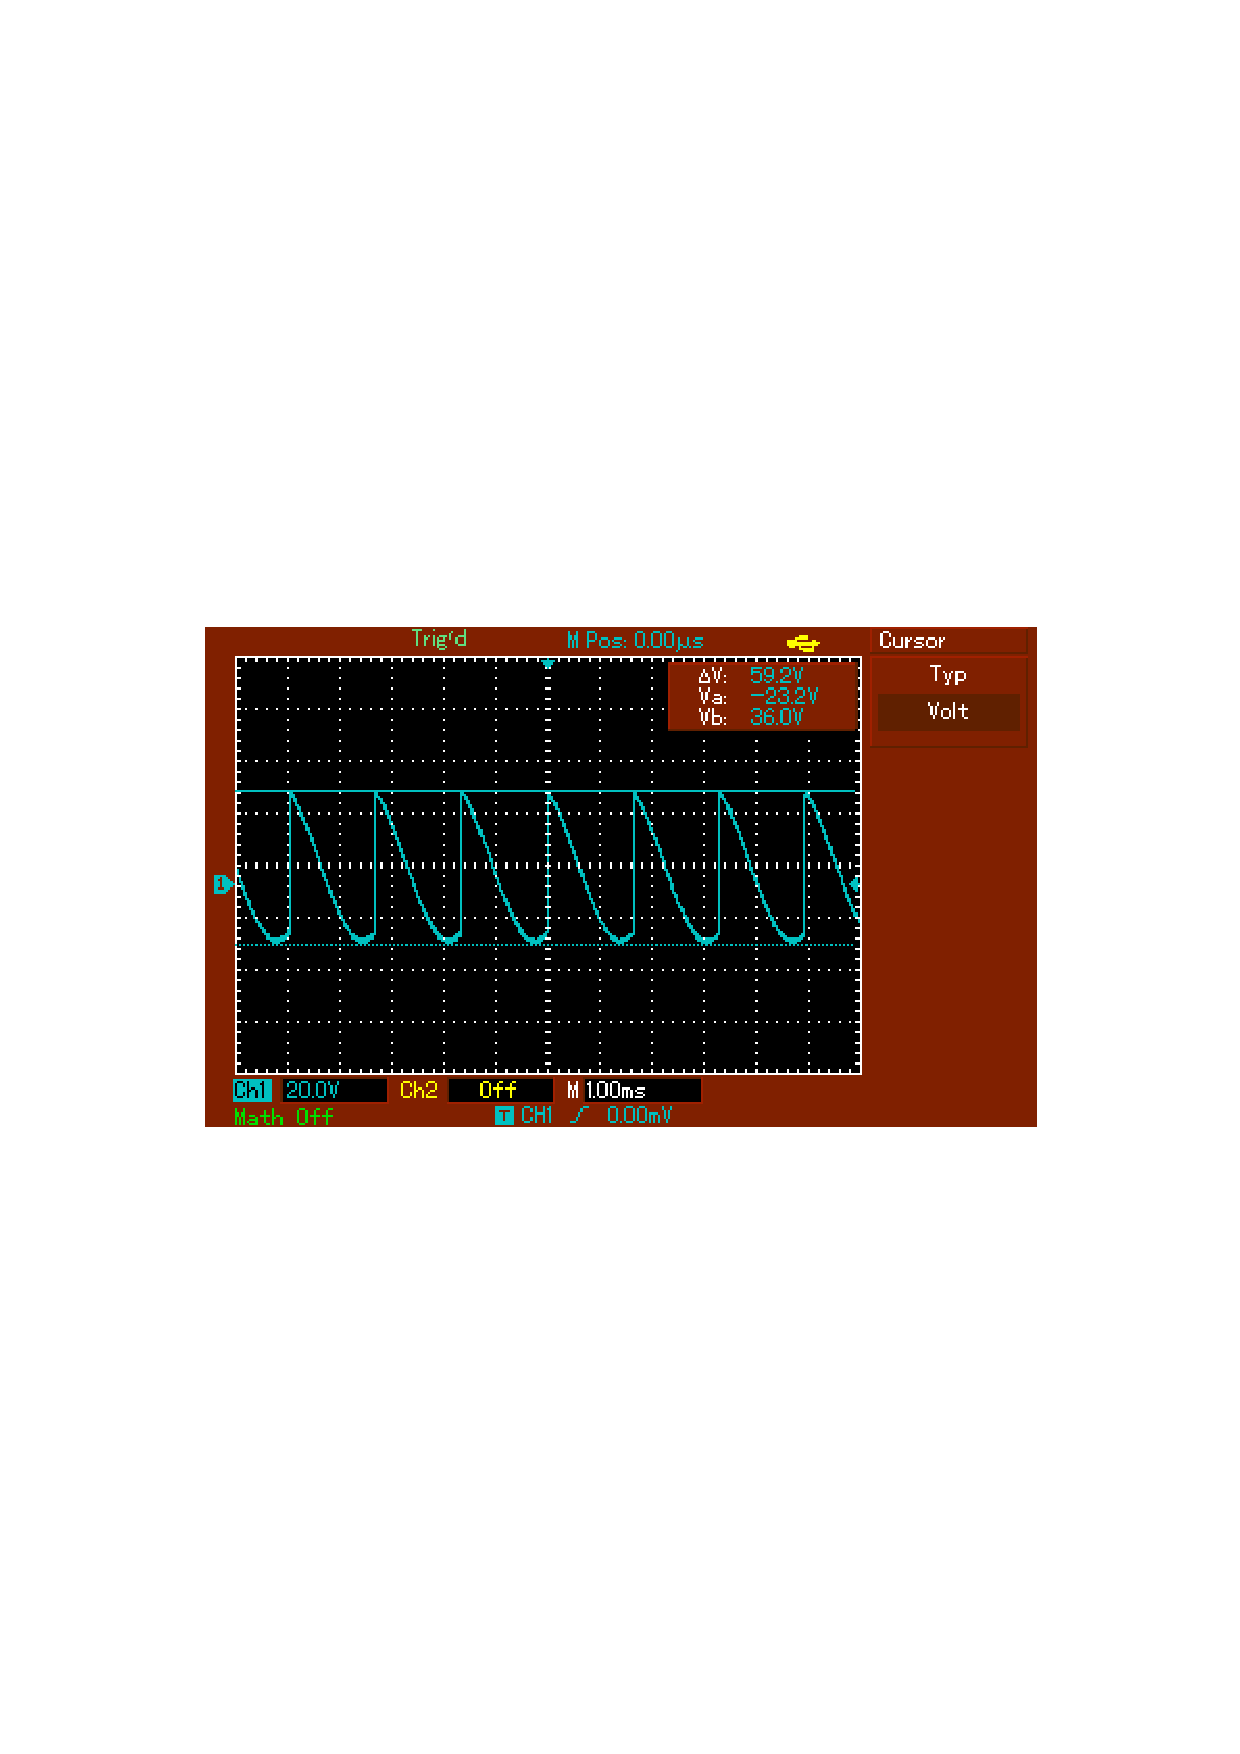
\includegraphics[height=4cm]{content/Bilder/unverrauscht/360.pdf}
    \caption{$\symup{\Delta}\varphi = \qty{360}{\degree}$}
  \end{subfigure}
  \caption{Oszilloskopbilder des Ausgabesignals $U_{\symup{sig}}$ für verschiedene Phasenverschiebungen $\symup{\Delta}\varphi$.}
  \label{fig:Bilder normal}
\end{figure}

Es zeigt sich, dass sich für das erste Bild \autoref{fig:unverrauscht 0} ein Spannungsverlauf passend zu dem in 
\autoref{fig:Signalverlaeufe} ergibt.
Aus den Bildern werden die jeweilgen Amplituden des Ausgabesignals für alle Phasenverschiebungen abgelesen und
in \autoref{tab:unverrauscht} festgehalten.

\begin{table} [H]
  \centering
  \caption{Amplitude des unverrauschten Signals in Abhängigkeit der Phasenverschiebung $\symup{\Delta}\varphi$}
  \label{tab:unverrauscht}
  \begin{tabular}{S[table-format=3.0] S[table-format=2.1]}
    \toprule
    {$\symup{\Delta}\varphi$} & {$U_{\symup{sig}}\,/\,\unit{\volt}$} \\
    \midrule
    0	  & 57.6 \\
    30	& 60.6 \\
    60	& 53.6 \\
    90	& 44.8 \\
    120	& 32.0 \\
    150	& 50.4 \\
    180	& 58.4 \\
    210	& 61.6 \\
    240	& 53.6 \\
    270	& 44.0 \\
    300	& 32.0 \\
    330	& 50.4 \\
    360	& 59.2 \\
    \bottomrule
  \end{tabular}
\end{table}

Diese Daten werden nun graphisch in \autoref{fig:plot normal} dargestellt und mit der Theoriekurve der Funktion 
\eqref{eq:Ausgangssignal Proportionalitaet} verglichen. Der Wert für die Spannung $U_{0}$ wird vorab zu $U_{0}=\qty{48}{\volt}$ 
gemessen.

\begin{figure} [H]
  \centering
  \includegraphics{build/plot_normal.pdf}
  \caption{Amplitude des Ausgangssignal $U_{\symup{sig}}$ vor dem Tiefpass in Abhängigkeit der Phasenverschiebung~$\varphi$.}
  \label{fig:plot normal}
\end{figure}

Ein Zusammenhang zwischen den Messwerten und der Theorie kann hier nicht bestätigt werden, möglich Gründe dafür werden in
der Diskussion genannt.

% Subsection mit Rauschen
\subsection{Messung mit Rauschen}
\label{sec:mit rauschen}

Es werden nun die Oszilloskopbilder betrachtet, die sich bei verrauschtem Eingangssignal ergeben haben.
Diese sind erneut für ausgewählte Phasenverschiebungen in \autoref{fig:Bilder rausch} zu sehen.

\begin{figure} [H]
  \begin{subfigure}{0.48\textwidth}
    \centering
    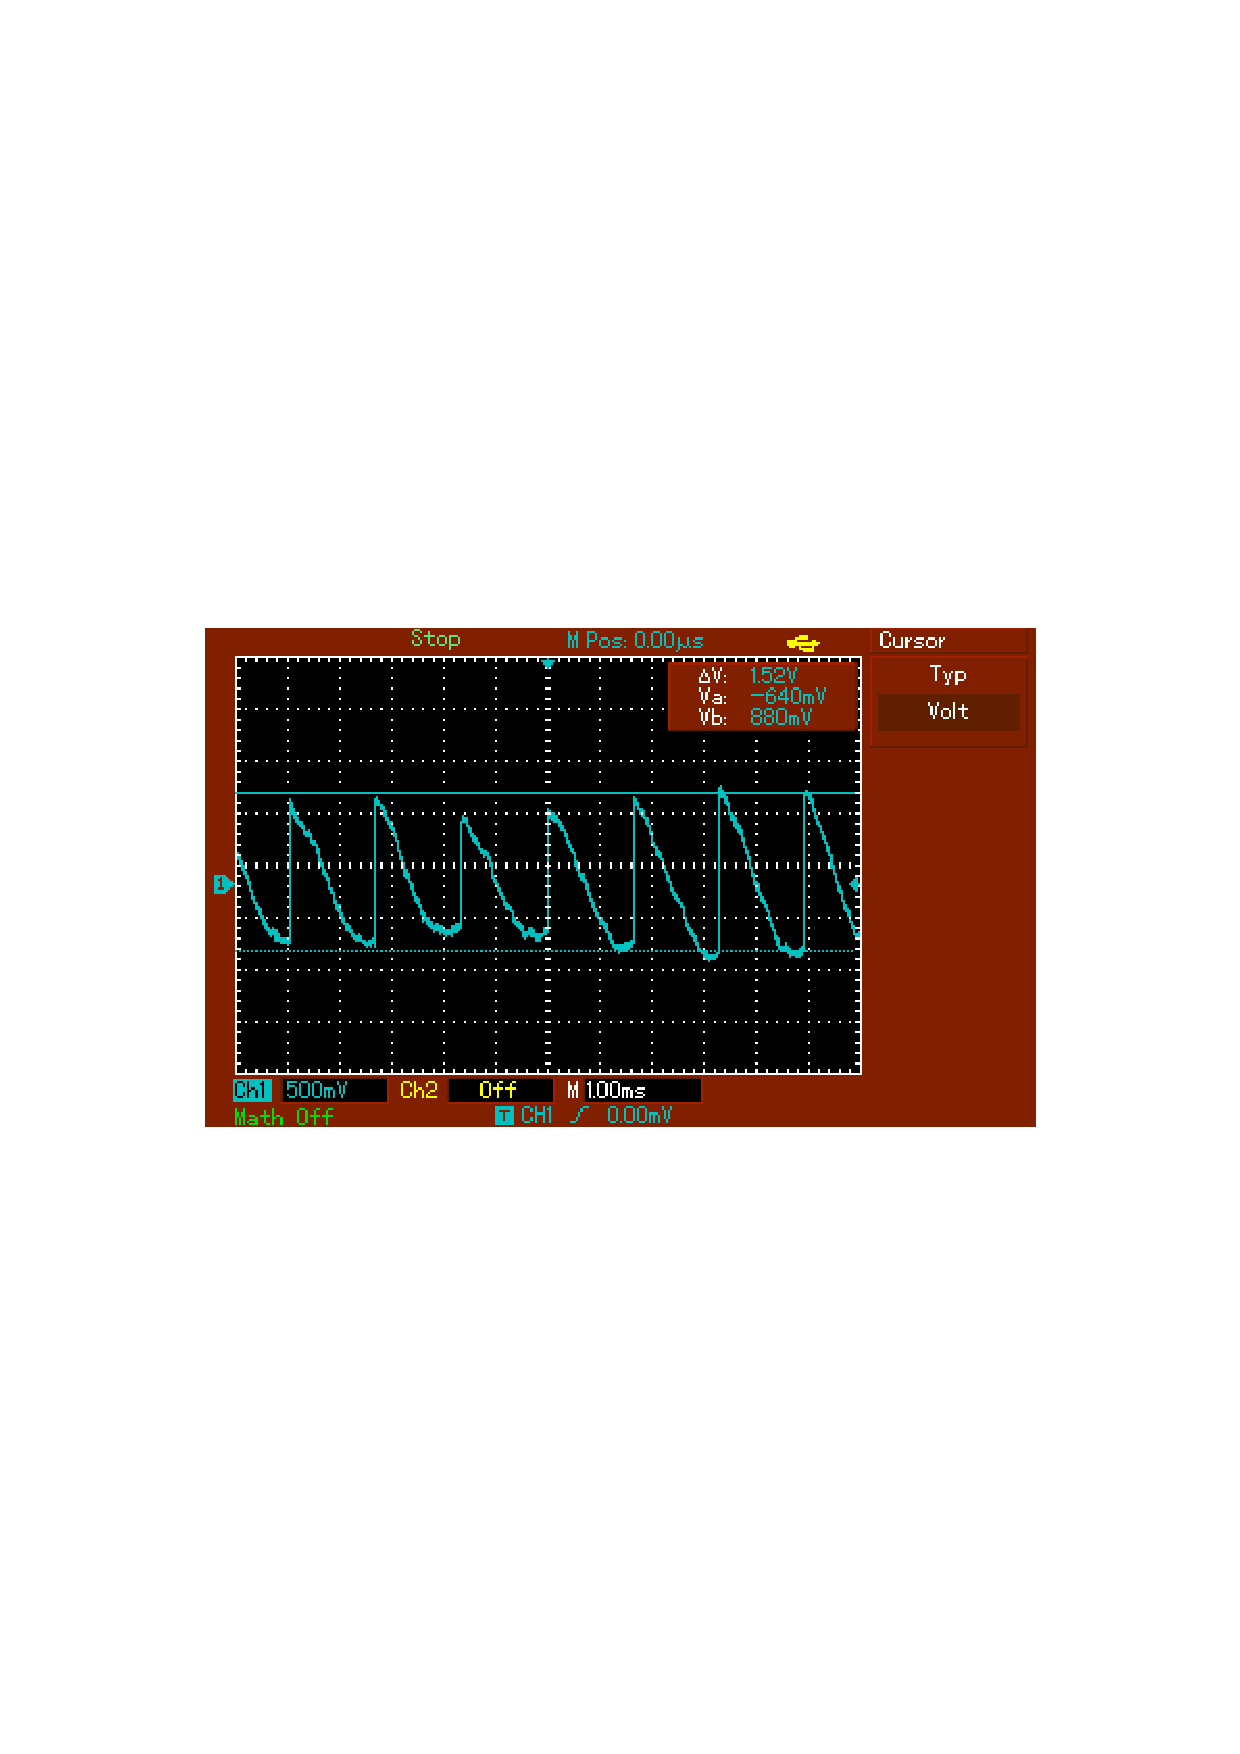
\includegraphics[height=4cm]{content/Bilder/verrauscht/0.pdf}
    \caption{$\symup{\Delta}\varphi = \qty{0}{\degree}$}
  \end{subfigure}
  \begin{subfigure}{0.48\textwidth}
    \centering
    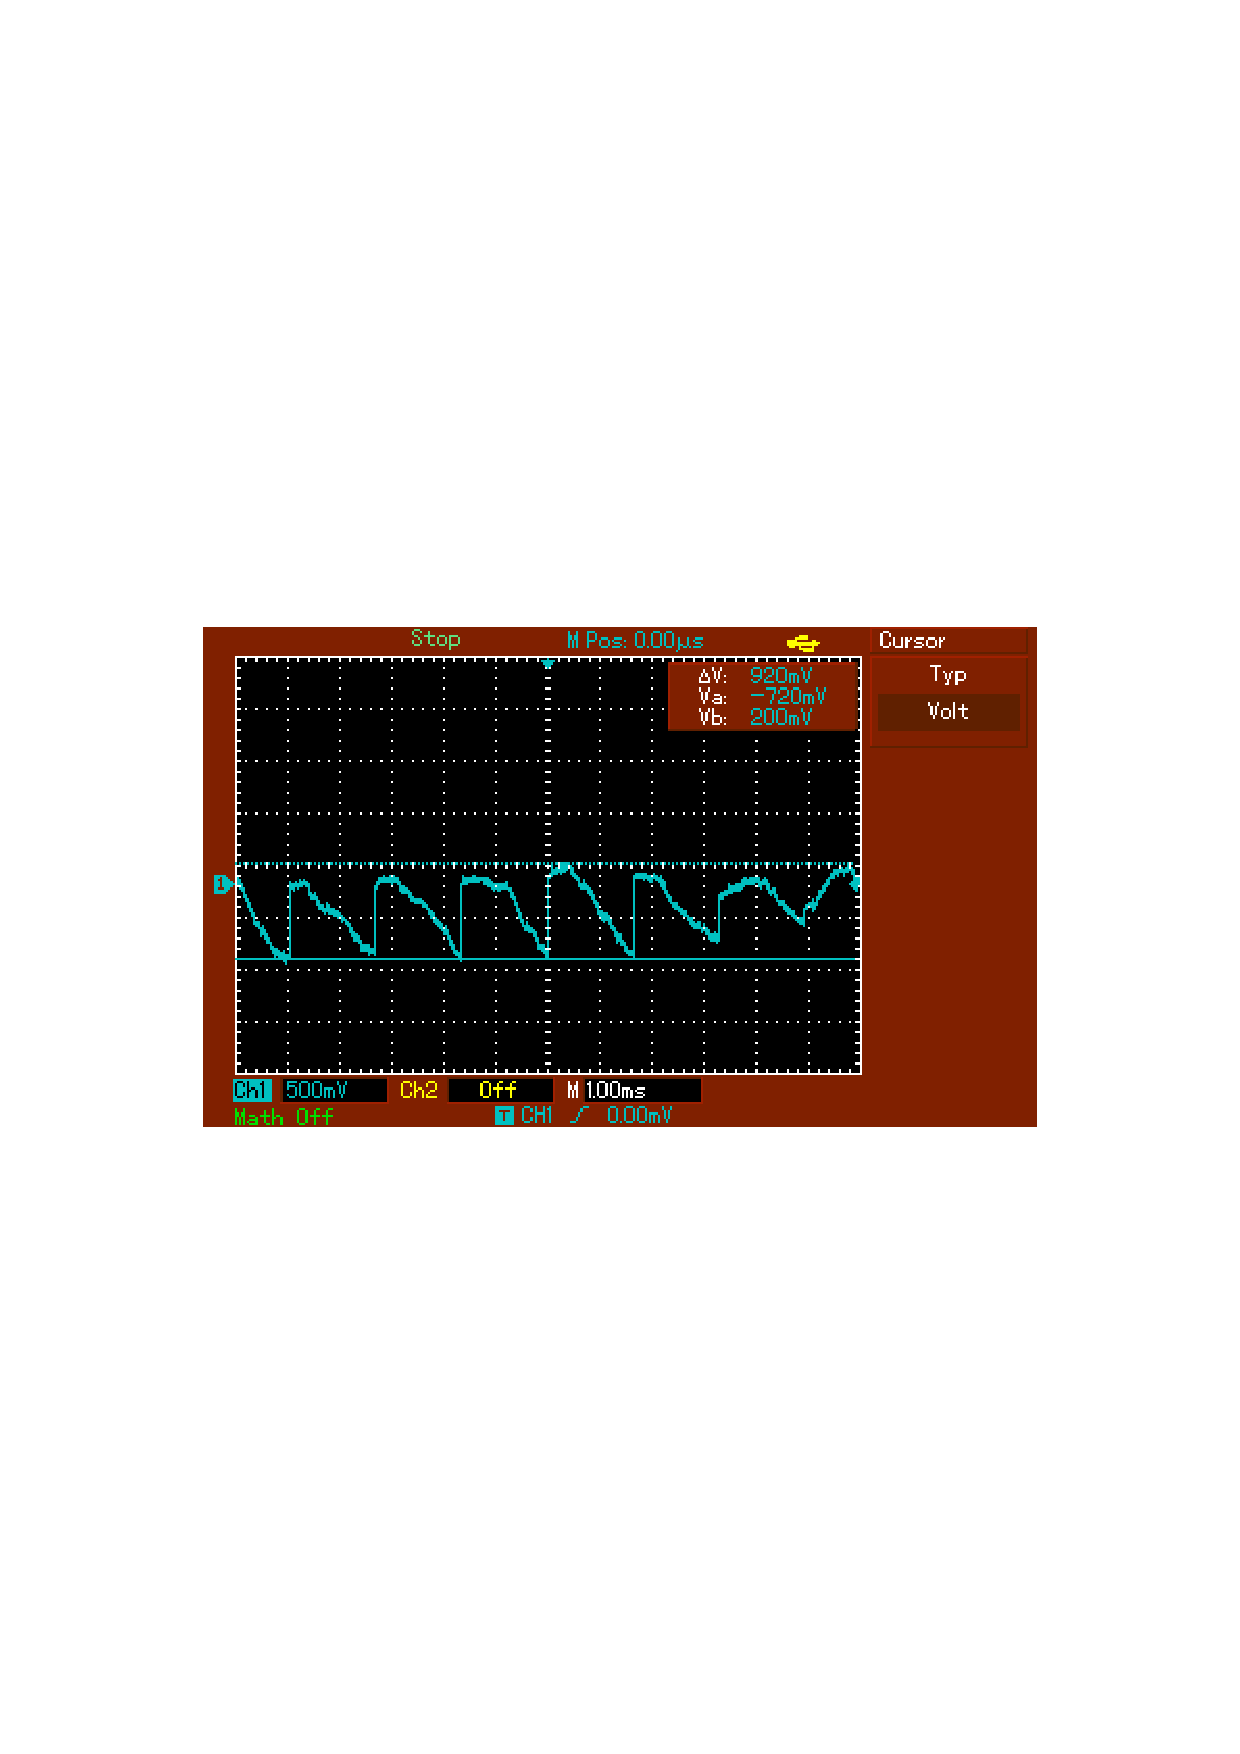
\includegraphics[height=4cm]{content/Bilder/verrauscht/90.pdf}
    \caption{$\symup{\Delta}\varphi = \qty{90}{\degree}$}
  \end{subfigure}
  \begin{subfigure}{0.48\textwidth}
    \centering
    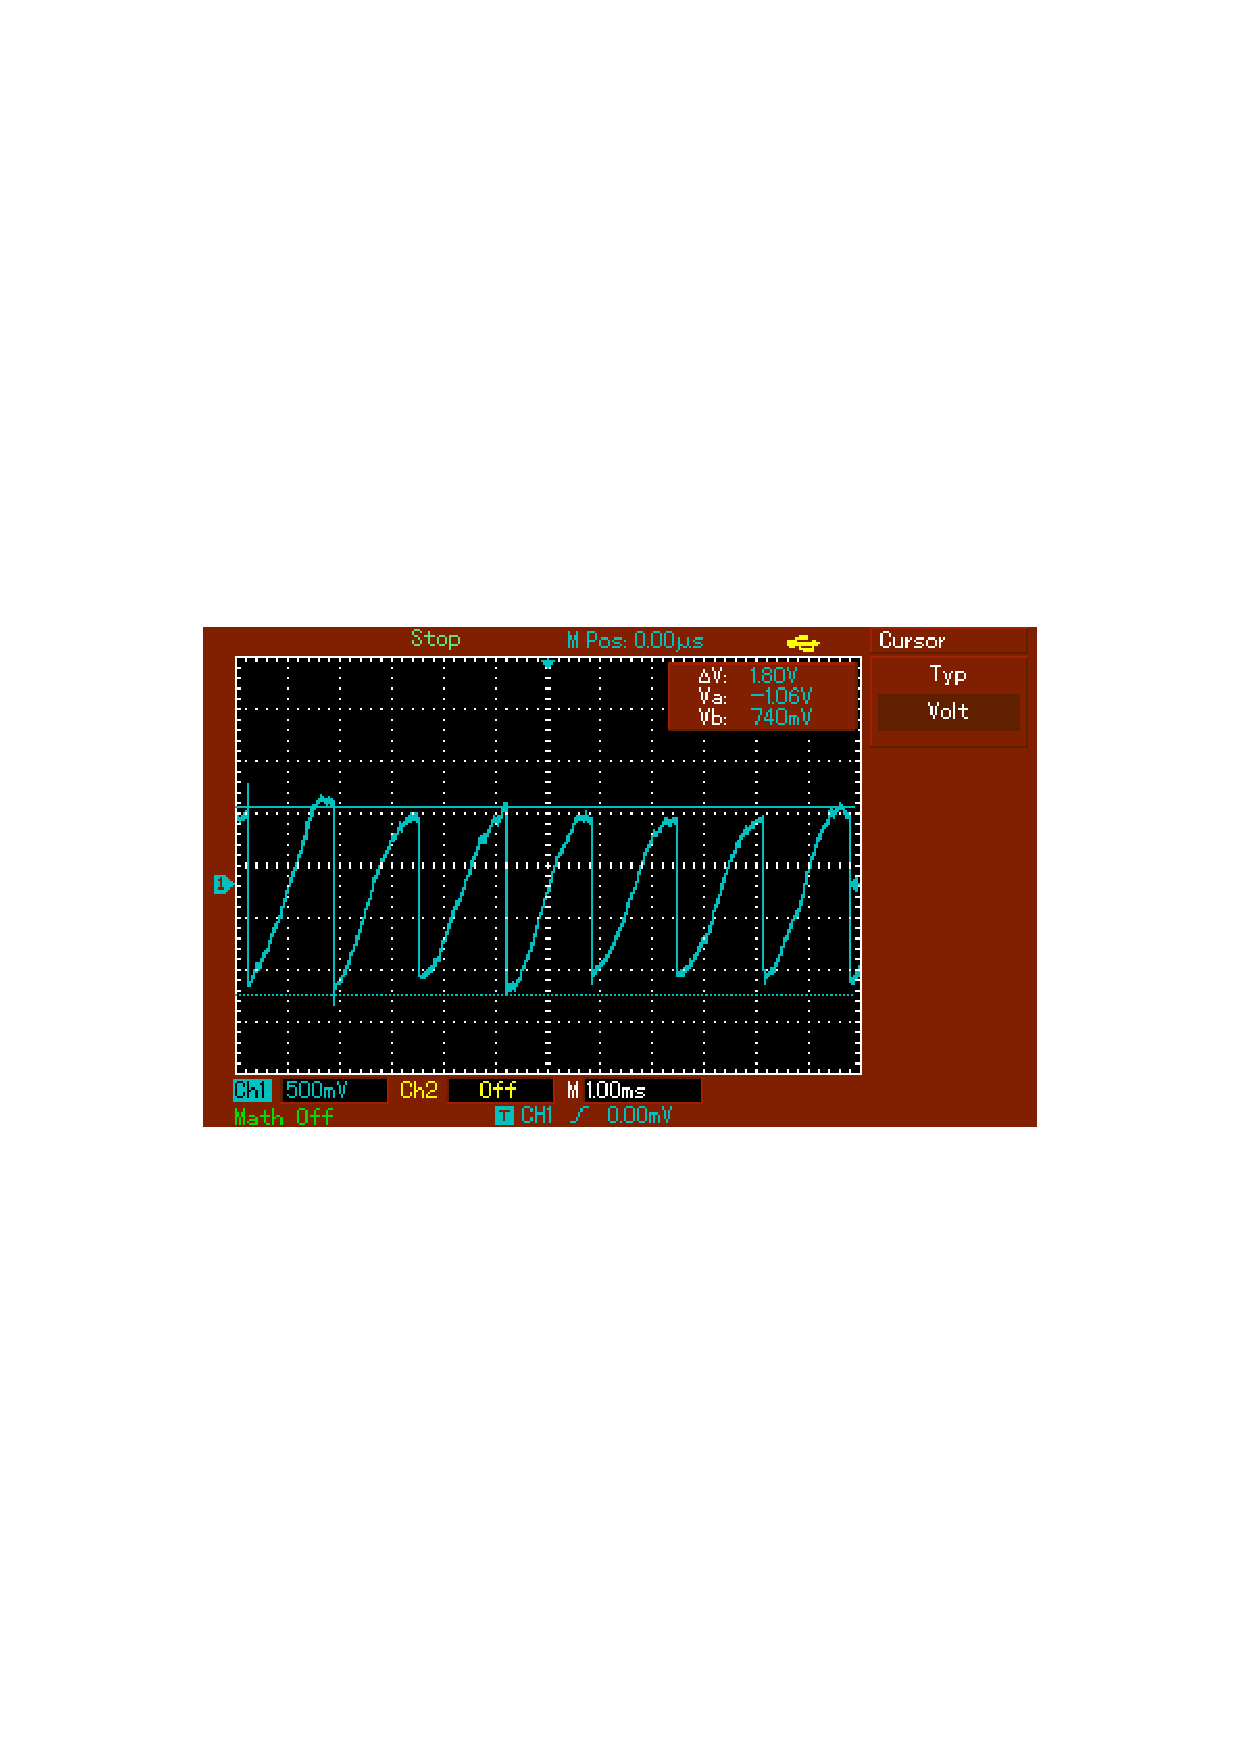
\includegraphics[height=4cm]{content/Bilder/verrauscht/180.pdf}
    \caption{$\symup{\Delta}\varphi = \qty{180}{\degree}$}
  \end{subfigure}
  \begin{subfigure}{0.48\textwidth}
    \centering
    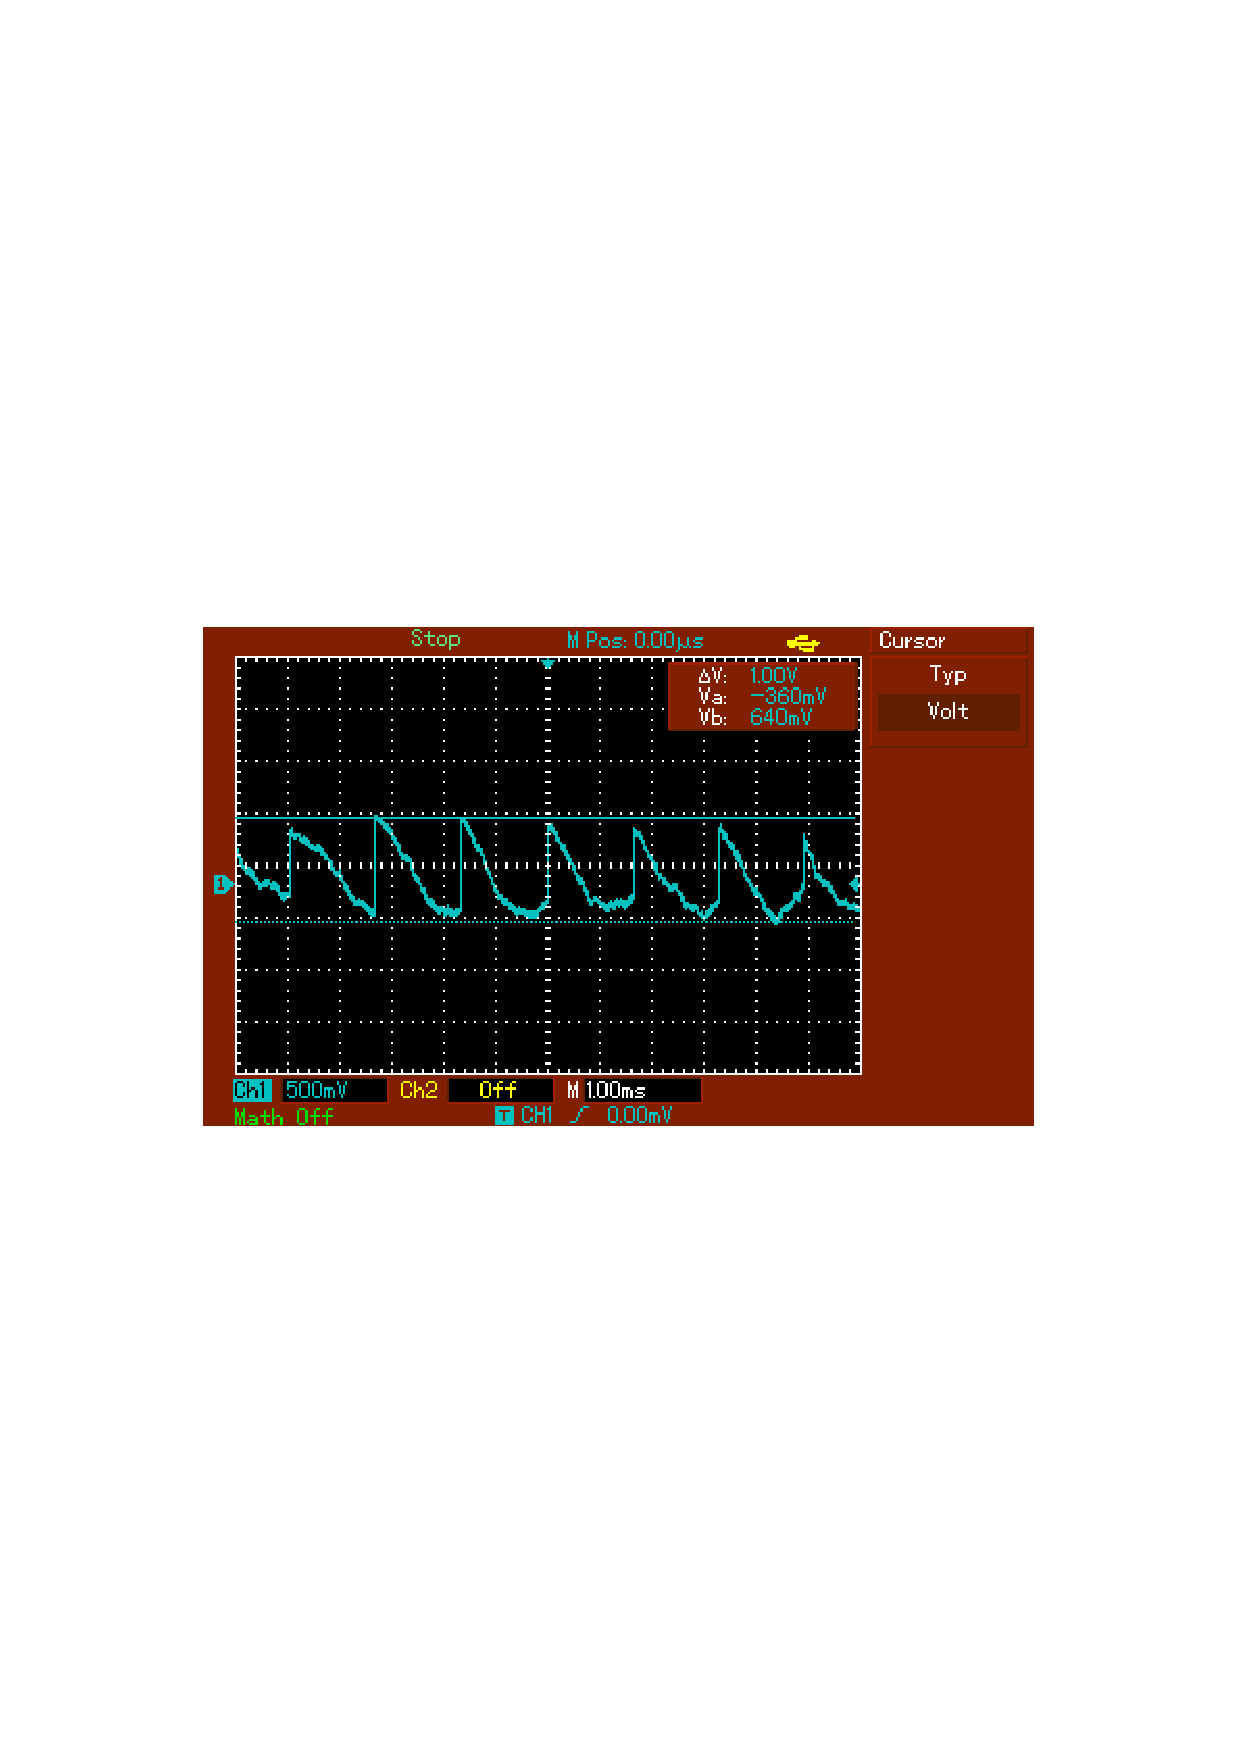
\includegraphics[height=4cm]{content/Bilder/verrauscht/270.pdf}
    \caption{$\symup{\Delta}\varphi = \qty{270}{\degree}$}
  \end{subfigure}
  \begin{subfigure}{0.48\textwidth}
    \centering
    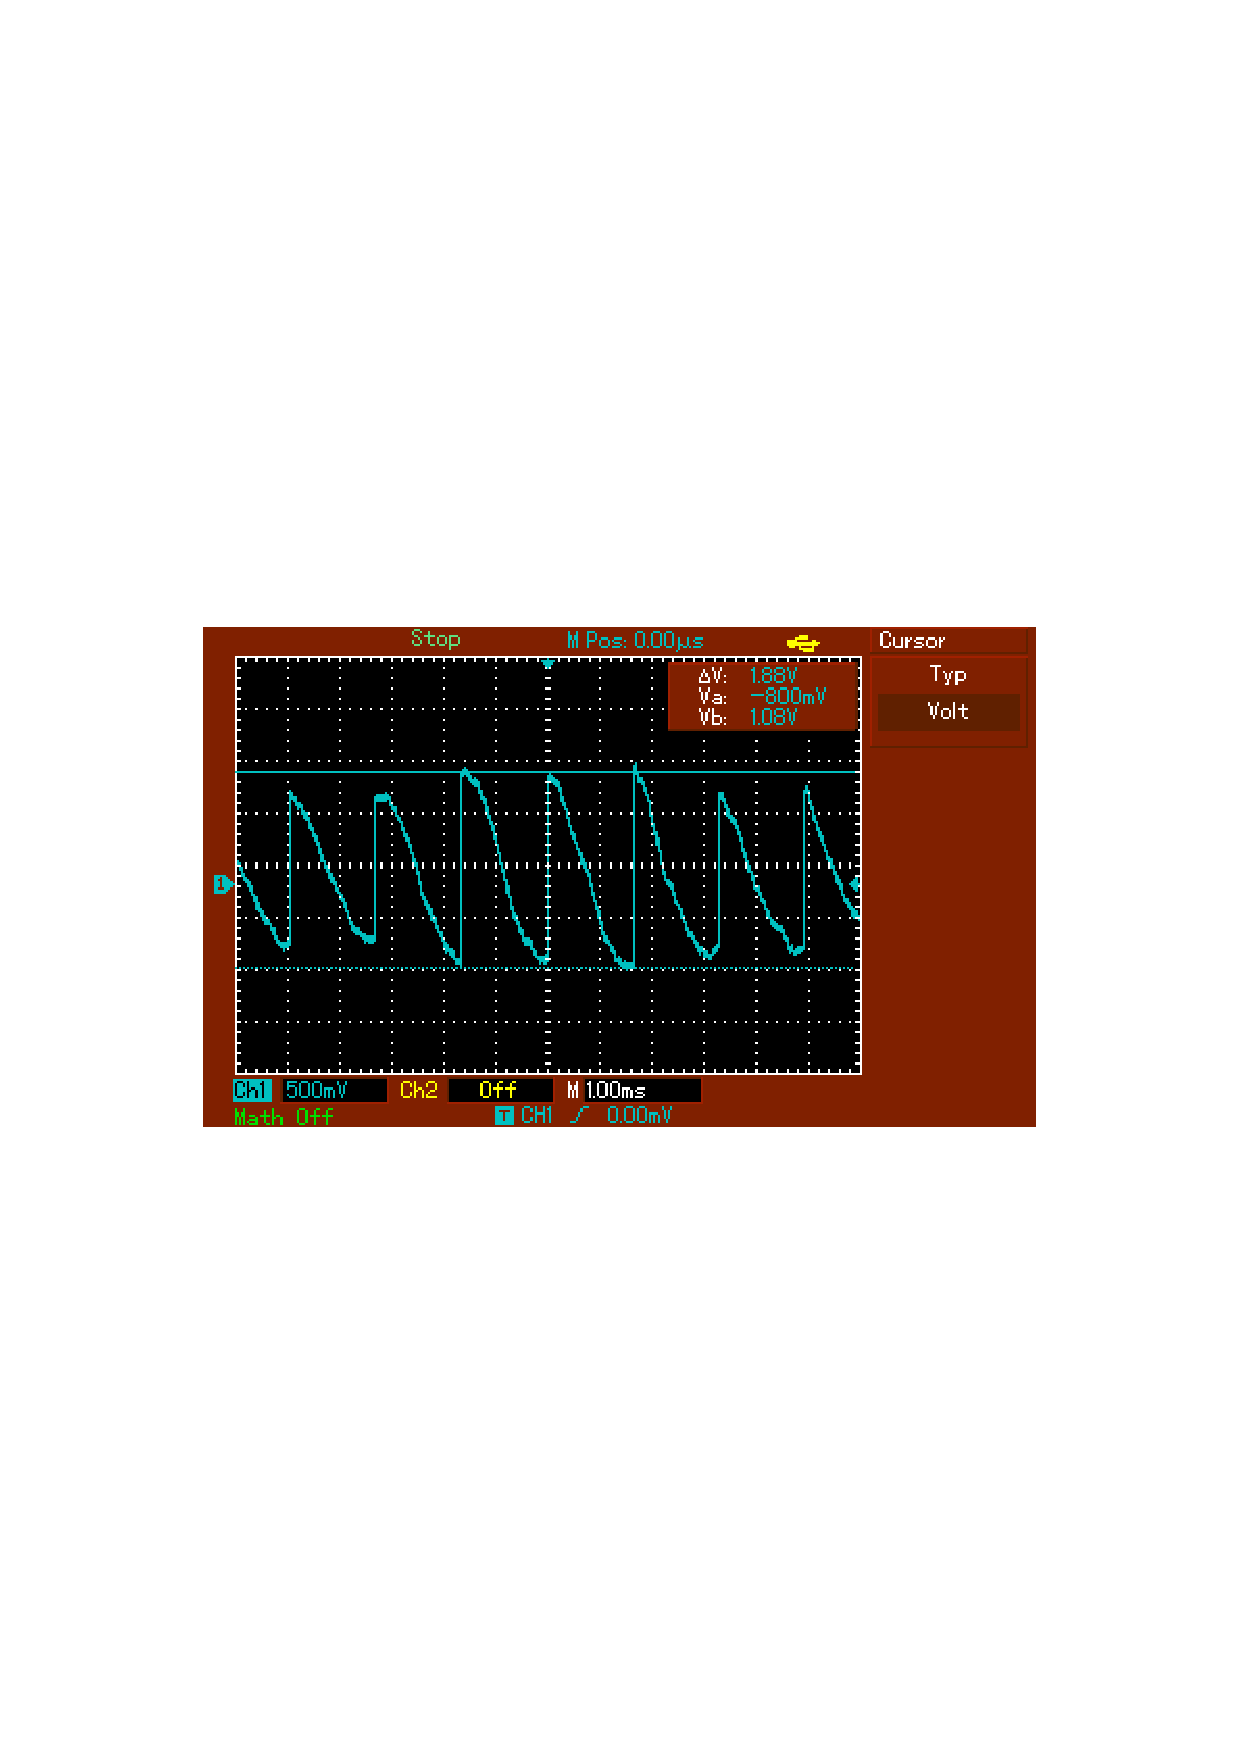
\includegraphics[height=4cm]{content/Bilder/verrauscht/360.pdf}
    \caption{$\symup{\Delta}\varphi = \qty{360}{\degree}$}
  \end{subfigure}
  \caption{Oszilloskopbilder des Ausgabesignals $U_{\symup{sig}}$ für verschiedene Phasenverschiebungen $\symup{\Delta}\varphi$ mit rauschen.}
  \label{fig:Bilder rausch}
\end{figure}

Vergleicht man die Oszilloskopbilder mit den Bildern in \autoref{fig:Bilder normal}, dann ist sofort
ein ähnlicher Signalverlauf zu erkennen.
Der Lock-In-Verstärker hat demnach wie erwartet das Rauschen größtenteils herausgefiltert und das Ausgangssignal
ist nährungsweise gleich geblieben.
Bei genauer Betrachtung fallen minimale Sprünge und kleine Unregelmäßigkeiten im Signalverlauf auf,
hier handelt es sich wahrscheinlich um besonders starke Störungen des Rauschgenerators, die der Lock-In-Verstärker
nicht vollständig herausfiltern konnte.

Insgesamt verifizieren die Bilder jedoch eindeutig die Funktionsweise des Lock-In-Verstärkers, anschließend
werden noch die Amplituden des Ausgabesignals analog zu \autoref{sec:ohne rauschen} in \autoref{tab:verrauscht} dargestellt.

\begin{table} [H]
  \centering
  \caption{Amplitude des verrauschten Signals in Abhängigkeit der Phasenverschiebung~$\symup{\Delta}\varphi$}
  \label{tab:verrauscht}
  \begin{tabular}{S[table-format=3.0] S[table-format=1.2]}
    \toprule
    {$\symup{\Delta}\varphi$} & {$U_{\symup{sig}}\,/\,\unit{\volt}$} \\
    \midrule
    0	  & 1.52 \\
    30	& 1.28 \\
    60	& 1.14 \\
    90	& 0.92 \\
    120	& 1.02 \\
    150	& 1.26 \\
    180	& 1.80 \\
    210	& 1.42 \\
    240	& 1.16 \\
    270	& 1.00 \\
    300	& 1.58 \\
    330	& 1.62 \\
    360	& 1.88 \\
    \bottomrule
  \end{tabular}
\end{table}

Die absoluten Werte der Amplituden sind hier deutlich geringer als die des unverrauschten Signals.
Deren Abhängigkeit von der Phasenverschiebung ist jedoch noch vergleichbar mit
der unverrauschten Messung in \autoref{tab:unverrauscht}.


% Subsection LED
\subsection{Messung mit einer LED}
\label{sec:LED}

Die gemessene Signalstärke $U_{\symup{out}}$ in Abhängigkeit des Abstandes $r$ ist in \autoref{tab:led} dokumentiert.

\begin{table} [H]
  \centering
  \caption{Signalstärke des Ausgabesignals des Photodetektors abhängig von dem Abstand $r$ zwischen LED und Photdetektor.}
  \label{tab:led}
  \begin{tabular}{S[table-format=2.1] S[table-format=3.1]}
    \toprule
    {$r\,/\,\unit{\centi\metre}$} & {$U_{\symup{sig}}\,/\,\unit{\volt}$} \\
    \midrule
    6.6	  & 210.0\\
    7.0	  & 194.0\\
    7.5	  & 170.0\\
    8.0	  & 138.0\\
    8.5	  & 110.0\\
    9.0	  & 93.6 \\
    9.5	  & 83.2 \\
    10.0	& 74.4 \\
    11.0	& 60.0 \\
    12.0	& 48.0 \\
    13.0	& 40.0 \\
    14.0	& 32.4 \\
    15.0	& 28.0 \\ 
    17.0	& 20.4 \\ 
    19.0	& 16.2 \\ 
    21.0	& 12.8 \\
    23.0	& 11.4 \\
    25.0	& 9.0  \\
    30.0	& 6.9  \\
    40.0	& 5.5  \\
    50.0	& 4.5  \\
    60.0	& 3.9  \\
    \bottomrule
  \end{tabular}
\end{table}

Die Werte werden in \autoref{fig:plot led} graphisch dargestellt.
Dazu wird eine nicht-lineare Ausgleichsfunktion mit \cite{scipy} bestimmt, um eine mögliche $\frac{1}{r^2}$-Abhängigkeit der
Signalstärke zu überprüfen. Dafür wird eine Funktion der Form:

\begin{equation}
  f(r)=\frac{C}{r^2} \notag
\end{equation}

als Ansatz verwendet.
Für den Parameter $C$ ergibt sich der Wert:

\begin{align}
  C &= \qty{8.63+-0.21}{\kilo\volt\square\centi\metre} \notag
\end{align}

Mit dem Fit lässt sich die $\frac{1}{r^2}$-Abhängigkeit gut bestätigen, in \autoref{fig:plot led} ist eine Korrelation
von Messwerten und Ausgleichsfunktion deutlich zu erkennen.
Somit ist die Funktionsweise des Lock-In-Verstärkers verifiziert, da das Rauschen des Umgebungslichtes erfolgreich herausgefiltert
werden konnte.

\begin{figure}
  \centering
  \includegraphics{build/plot_led.pdf}
  \caption{Amplitude der Signalstärke $U_{\symup{sig}}$ des Photodetektors abhängig von dem Abstand $r$ zwischen der LED und des Photodetektors.}
  \label{fig:plot led}
\end{figure}
